\documentclass[dvipdfmx,autodetect-engine,10pt,b5paper,papersize,openany,dvipsnames]{jsbook}


\usepackage{color}
\usepackage{titlesec}
\usepackage{multicol}

% 本文をゴシックに
\usepackage[deluxe]{otf}
\renewcommand{\kanjifamilydefault}{\gtdefault}
\renewcommand{\familydefault}{\sfdefault}

\usepackage{amsmath,txfonts}
\usepackage{bm}
\usepackage{mathrsfs} % \mathscr

\usepackage[dvipdfmx]{graphicx}

% PDF を読み込み
\usepackage{pdfpages}

\usepackage{fancyhdr}

\usepackage{tikzpagenodes}
%\usepackage[object=vectorian]{pgfornament}
\usetikzlibrary{shapes.geometric,calc}


% AddToShipoutPictureBG*
\usepackage{eso-pic}


%\usepackage[dvipdfmx]{hyperref}
\usepackage[hidelinks]{hyperref}
\usepackage{pxjahyper}


\usepackage{listings}
\lstset{
  title={},
  caption={},
  frame={single},
  numbers=none,
  lineskip=-0.5ex,
  basicstyle={\small\ttfamily},
  identifierstyle={\small},
  commentstyle={\smallitshape},
  keywordstyle={\small\bfseries},
  ndkeywordstyle={\small},
  stringstyle={\small\ttfamily},
}

% https://oku.edu.mie-u.ac.jp/~okumura/jsclasses/
% jsbook の余白が広すぎます
% 書籍では1行の長さが全角40文字を超えないようにしています。
% そのため,段組をしないときは,自動的にどちらかの余白が広くなります
% (美文書シリーズのようなデザインになります)。
% これが困るときはプリアンブル(\begin{document} の前)に次のように書いてください。
\setlength{\textwidth}{\fullwidth}
\setlength{\evensidemargin}{\oddsidemargin}

% for \ruby{}{}
\usepackage{okumacro}

% 奥付
\newcommand{\bhline}[1]{\noalign{\hrule height #1}}

\title{
  \textbf{月刊 ZENKEI AI MAGAZINE\\
  2021年5月号}
}
\author{\textbf{\textsf{ZENKEI AI FORUM}}}
\date{}

\pagestyle{fancy}
\fancyhf{} % 既定設定をリセット
\renewcommand{\headrulewidth}{0pt} % 罫線無し
\fancyfoot[C]{\thepage}

\AtBeginDocument{
  \addtocontents{toc}{\protect\thispagestyle{fancy}}
}

\begin{document}

%\maketitle


%\thispagestyle{fancy}
%\setcounter{page}{1}
\AddToShipoutPictureBG*{%
  \AtPageLowerLeft{%
    \includegraphics[width=\paperwidth,height=\paperheight]%
      {images/20210628_2_l_TOC.jpg}
  }%
}%

%\tableofcontents
\thispagestyle{empty}
 % 全角空白

\newpage

\thispagestyle{fancy}
\setcounter{page}{1}
\AddToShipoutPictureBG*{%
  \AtPageLowerLeft{%
    \includegraphics[width=\paperwidth,height=\paperheight]%
      {images/20210628_2_r.jpg}
  }%
}%

 % 全角空白

\newpage

\AddToShipoutPictureBG*{%
  \AtPageLowerLeft{%
    \includegraphics[width=\paperwidth,height=\paperheight]%
      {images/20210628_3_l.jpg}
  }%
}%

\chapter*{まえがき}
\addcontentsline{toc}{chapter}{まえがき}
\thispagestyle{fancy}
\begin{tikzpicture}[
  remember picture, overlay]
\node[yshift=-8em,yscale=1.2,xslant=0.25,color=Gray] (text)
  at (current page.north){%
  \sffamily \large
  【月刊 ZENKEI AI MAGAZINE 2021年5月号】};
\end{tikzpicture}

月刊 ZENKEI AI MAGAZINE (ZAM) の5月号です。
今年の2021年1月にスタートしてから本号で4冊目になります。
はい、実はまだ4月号が完成していません
(ZENKEI AI FORUM 4月の回は市來の一人喋りになったため、
  執筆者が私だけなので、発行が遅れて悲しいのも私だけ)。
ということで、予定通り刊行される『月刊 ZAM 5月号』です。
お楽しみください!


\begin{flushright}
  2021年6月30日\\
  金沢にて\\
  ZENKEI AI MAGAZINE 編集長\\
  市來健吾
\end{flushright}

\begin{tikzpicture}[remember picture, overlay]
  \begin{scope}[thick,rounded corners=8pt,
      line width=16pt,
      xscale=1.3, yscale=1.3, xshift=-1.75cm, yshift=-5.0cm]
  \draw (0, 2) -- (5, 2) -- (4, 0) [sharp corners] -- (5.5, 0)
    [rounded corners=8pt] -- (6.5, 2) [sharp corners] -- (7.5, 0)
    -- (8.5, 0);
  \draw (3.5, 0.8) -- (7.5, 0.8)
    -- (8.2, 2) -- (9.2, 0) -- (10.2, 2) -- (10.2, 0) -- (14, 0);
  \end{scope}
\end{tikzpicture}


\newpage

\AddToShipoutPictureBG*{%
  \AtPageLowerLeft{%
    \includegraphics[width=\paperwidth,height=\paperheight]%
      {images/20210628_3_r.jpg}
  }%
}%

\chapter{当日のイベントの模様}
\label{sec:introduction}
\thispagestyle{fancy}

5月の ZENKEI AI FORUM (ZAF)  は2021年5月26日に開催されました。
当日の模様は YouTube のアーカイブ (\url{https://youtu.be/GwbYxcMWa7w})
でご覧になれますので、見逃した方はそちらでご覧ください。
この日はゲスト3名お迎えしました。
ZAM 本号の内容はこの ZAF をベースにして、
以下のような構成になります。
\begin{itemize}
\item \textgt{\bfseries \sffamily
  【第 \ref{ch:furukawa} 章】 アイリス VS ペンギン (furukawa)}\\
  『ゼロからはじめるAI』シリーズの furukawa さんに、
  機械学習で使われるデータセットの最近のはなしを紹介していただきます。
\item \textgt{\bfseries \sffamily
  【第 \ref{ch:ishikawa} 章】 Kaggle 奮闘記(石川達也)}\\
  全景株式会社で AI モデルなど開発している石川さんに、
  先日挑戦して結構いいところまで行ったという Kaggle のはなしです。
\item \textgt{\bfseries \sffamily
  【第 \ref{ch:yoneda} 章】 ZENKEI AI FORUMへの提言(米田稔)}\\
  前回4月の ZAF でいただいたコメントを発端に
  「社会に役に立つ ZENKEI AI FORUM」という視点でおはなしをしていただきます。
\end{itemize}


\newpage

\titleformat{\chapter}[block]
{} % style
{} % label
{0pt} % spacing
{} % in front of the title
[]
\chapter[アイリス VS ペンギン (furukawa)]{}
\label{ch:furukawa}

\pagestyle{fancy}
\fancyhf{} % 既定設定をリセット
\renewcommand{\headrulewidth}{0pt} % 罫線無し
\fancyfoot[RE]{第2章 アイリス VS ペンギン}
\fancyfoot[LO]{furukawa}
\fancyfoot[LE,RO]{\thepage}

\thispagestyle{fancy}

\AddToShipoutPictureBG*{%
  \AtPageLowerLeft{%
    \includegraphics[width=\paperwidth,height=\paperheight]%
      {images/20210620_iris_vs_penguins-nup1x2-p1-90percent.png}
  }%
}%

%\includepdf[pages=2-10, pagecommand={}]%
\includepdf[scale=0.9, pages=3-, nup=1x2, pagecommand={}]%
  {20210620_iris_vs_penguins.pdf}

\newpage

\titleformat{\chapter}[block]
{} % style
{} % label
{0pt} % spacing
{} % in front of the title
[]
\chapter[Kaggle 奮闘記(石川達也)]{}
\label{ch:ishikawa}

\pagestyle{fancy}
\fancyhf{} % 既定設定をリセット
\renewcommand{\headrulewidth}{0pt} % 罫線無し
\fancyfoot[RE]{第3章 Kaggle 奮闘記}
\fancyfoot[LO]{石川達也}
\fancyfoot[LE,RO]{\thepage}

\thispagestyle{fancy}

\AddToShipoutPictureBG*{%
  \AtPageLowerLeft{%
    \includegraphics[width=\paperwidth,height=\paperheight,page=1]%
      {20210627_Kaggel奮闘記.pdf}
  }%
}%

%\includepdf[pages=2-10, pagecommand={}]%
%\includepdf[scale=0.9, pages=1-, pagecommand={}]%
\includepdf[pages=2-, pagecommand={}]%
  {20210627_Kaggel奮闘記.pdf}

\newpage

\titleformat{\chapter}[block]
{} % style
{} % label
{0pt} % spacing
{} % in front of the title
[]
\chapter[ZENKEI AI FORUMへの提言(米田稔)]{}
\label{ch:yoneda}

\pagestyle{fancy}
\fancyhf{} % 既定設定をリセット
\renewcommand{\headrulewidth}{0pt} % 罫線無し
\fancyfoot[RE]{第4章 ZENKEI AI FORUMへの提言}
\fancyfoot[LO]{米田稔}
\fancyfoot[LE,RO]{\thepage}

\thispagestyle{fancy}

\AddToShipoutPictureBG*{%
  \AtPageLowerLeft{%
    \includegraphics[width=\paperwidth,height=\paperheight]%
      {images/ZAM2021SumMY-p1-90percent.png}
  }%
}%

\includepdf[scale=0.9, pagecommand={}]%
  {ZAM2021SumMY_P2.pdf}

\newpage

\includepdf[scale=0.9, pages=3-, pagecommand={}]%
  {ZAM2021SumMY.pdf}

\newpage

\AddToShipoutPictureBG*{%
  \AtPageLowerLeft{%
    \includegraphics[width=\paperwidth,height=\paperheight]%
      {images/20210628_3_r.jpg}
  }%
}%

 % 全角空白

\newpage

\AddToShipoutPictureBG*{%
  \AtPageLowerLeft{%
    \includegraphics[width=\paperwidth,height=\paperheight]%
      {images/20210628_3_r.jpg}
  }%
}%

\titleformat{\chapter}[block]
{\gtfamily \Huge} % style
{} % label
{0pt} % spacing
{} % in front of the title
[]
\chapter*{執筆者紹介}
\addcontentsline{toc}{chapter}{執筆者紹介}

\pagestyle{fancy}
\fancyhf{} % 既定設定をリセット
\renewcommand{\headrulewidth}{0pt} % 罫線無し
\fancyfoot[RE]{執筆者紹介}
\fancyfoot[LO]{\rightmark}
\fancyfoot[LE,RO]{\thepage}

\thispagestyle{fancy}

{\small
今月の執筆者紹介です。

\subsection*{第 \ref{sec:introduction} 章\\ \ruby{市來}{いちき}\ruby{健吾}{けんご} (ZAM 編集長)}

自分とみんなの人生が楽しくなるかなと思って、
勝手に雑誌を作って、勝手に編集長をやっています。

結局いつも自分の原稿が一番遅いですね。

\begin{tikzpicture}[remember picture, overlay]
  %\node[xshift=1.0cm,yshift=1.3cm] at (current page.west){
  \node[xshift=-0.9cm,yshift=1.3cm] at (current page.east){
    \includegraphics[width=0.12\textwidth]%
      {images/editor-in-chief.png}
  };
  %\node[xshift=1.0cm,yshift=-2.0cm] at (current page.west){
  \node[xshift=-0.9cm,yshift=-2.0cm] at (current page.east){
    \includegraphics[width=0.12\textwidth]%
      {images/aiforum_20210628_1.jpg}
  };
  %\node[xshift=1.0cm,yshift=-5.0cm] at (current page.west){
  \node[xshift=-0.9cm,yshift=-5.0cm] at (current page.east){
    \includegraphics[width=0.12\textwidth]%
      {images/ishikawa.png}
  };
  %\node[xshift=1.0cm,yshift=-8.8cm] at (current page.west){
  \node[xshift=-0.9cm,yshift=-8.8cm] at (current page.east){
    \includegraphics[width=0.12\textwidth]%
      {images/ProfPhotoS_edit2.jpg}
  };
\end{tikzpicture}

\subsection*{第 \ref{ch:furukawa} 章\\ furukawa (全景株式会社)}

職業:エンジニア、趣味:お絵描き

かわいいものが好きです。

\subsection*{第 \ref{ch:ishikawa} 章\\ \ruby{石川}{いしかわ}\ruby{達也}{たつや}(全景株式会社)}

1991年生まれ、愛知県出身。金沢大学大学院自然科学研究科数物科学専攻(旧 物理学部)修士課程終了。
愛知で自動車の組み込み系の開発に従事し、なんだかんだあってで金沢に戻って来ました。
現在は全景株式会社でプログラマをしています。AIは勉強し始めて1年くらい。


\subsection*{第 \ref{ch:yoneda} 章\\ \ruby{米田}{よねだ}\ruby{稔}{みのる}(株式会社COM-ONE 代表取締役社長)}

石川高専卒後コマツソフト、コマツパキスタンソフト(イスラマバード)勤務を経て、
2003年に株式会社COM-ONEを設立し現在に至る。
ZENKEI AI FORUM の前身であるZENKEI AI SEMINAR からのメンバー。
}
\begin{tikzpicture}[
  remember picture, overlay]
\node[yshift=-8em,yscale=1.2,xslant=0.25,color=Gray] (text)
  at (current page.north){%
  \sffamily \large
  【月刊 ZENKEI AI MAGAZINE 2021年5月号】};
\end{tikzpicture}

\newpage

\AddToShipoutPictureBG*{%
  \AtPageLowerLeft{%
    \includegraphics[width=\paperwidth,height=\paperheight]%
      {images/20210628_3_r.jpg}
  }%
}%

\chapter*{編集後記}
\addcontentsline{toc}{chapter}{編集後記}

\pagestyle{fancy}
\fancyhf{} % 既定設定をリセット
\renewcommand{\headrulewidth}{0pt} % 罫線無し
\fancyfoot[RE]{\leftmark}
\fancyfoot[LO]{編集後記}
\fancyfoot[LE,RO]{\thepage}

\thispagestyle{fancy}

今月号(2021年5月号)の刊行は、予定通り、
ZENKEI AI FORUM 6月のイベントの日(2021年6月30日開催予定)に間に合いました。

と言っても(まえがきに書いた通り)実は1つ前の『月刊 ZAM 4月号』がまだ出来上がってません。
(これからがんばります。)

いつものことですが、執筆者の3名のみなさまには、
きちんと原稿をいただきました。ありがとうございました。
いろいろな人の書いたものが1冊の本になるのが、やっぱり雑誌の醍醐味ですね。

\vspace{1em}

ところで来月の7月は ZENKEI AI FORUM もサークルとして過去2回参加した
技術同人誌イベント『技術書典11』が開催されます。
私たちも今回も引き続き出典予定です。
既刊の単行本(furukawa さんの『\href{https://techbookfest.org/product/6566174659706880}{ゼロからはじめるAI}』や中野裕さんの『\href{https://techbookfest.org/product/5840767786418176}{Jupyter BookでAIの解説本を書く方法}』ほか)に加え、目玉は ZAM の有料版である『ZAM 季報』の創刊です。
予定では『月刊 ZAM』の1月号から6月号までの内容をベースに、
サークルメンバーによる書き下ろしコンテンツを加えて、
魅力ある雑誌にしたいと考えています。
みなさま是非ご参加ください!

\vspace{1em}

今月号の表紙デザインおよび口絵のイラストは、
『月刊 ZAM 2月号』でも表紙デザインしてもらった furukawa さんです。


\begin{flushright}
  (市來健吾)
\end{flushright}

% rainbow
\begin{tikzpicture}[remember picture, overlay,
    %xscale=1.5, yscale=1.5, xshift=-2.5cm, yshift=-5cm]
    xscale=1.5, yscale=1.5, xshift=-2.5cm, yshift=-2cm]
  \begin{scope}[thick, rounded corners=8pt,color=red]
  \draw (0, 2) -- (5, 2) -- (4, 0) -- (5.5, 0);
  \draw (5.5, 0) -- (6.5, 2) -- (7.5, 0);
  \draw (7.5, 0) -- (8.5, 0);
  \draw (3.5, 0.8) -- (7.5, 0.8)
    -- (8.2, 2) -- (9.2, 0) -- (10.2, 2) -- (10.2, 0) -- (14, 0);
  \end{scope}

  \begin{scope}[thick, rounded corners=8pt,color=orange,
      xshift=0.04cm,yshift=-0.1cm]
  \draw (0, 2) -- (5, 2) -- (4, 0) -- (5.5, 0);
  \draw (5.5, 0) -- (6.5, 2) -- (7.5, 0);
  \draw (7.5, 0) -- (8.5, 0);
  \draw (3.5, 0.8) -- (7.5, 0.8)
    -- (8.2, 2) -- (9.2, 0) -- (10.2, 2) -- (10.2, 0) -- (14, 0);
  \end{scope}

  \begin{scope}[thick, rounded corners=8pt,color=yellow,
      xshift=0.08cm,yshift=-0.2cm]
  \draw (0, 2) -- (5, 2) -- (4, 0) -- (5.5, 0);
  \draw (5.5, 0) -- (6.5, 2) -- (7.5, 0);
  \draw (7.5, 0) -- (8.5, 0);
  \draw (3.5, 0.8) -- (7.5, 0.8)
    -- (8.2, 2) -- (9.2, 0) -- (10.2, 2) -- (10.2, 0) -- (14, 0);
  \end{scope}

  \begin{scope}[thick, rounded corners=8pt,color=green,
      xshift=0.12cm,yshift=-0.3cm]
  \draw (0, 2) -- (5, 2) -- (4, 0) -- (5.5, 0);
  \draw (5.5, 0) -- (6.5, 2) -- (7.5, 0);
  \draw (7.5, 0) -- (8.5, 0);
  \draw (3.5, 0.8) -- (7.5, 0.8)
    -- (8.2, 2) -- (9.2, 0) -- (10.2, 2) -- (10.2, 0) -- (14, 0);
  \end{scope}

  \begin{scope}[thick, rounded corners=8pt,color=blue,
      xshift=0.16cm,yshift=-0.4cm]
  \draw (0, 2) -- (5, 2) -- (4, 0) -- (5.5, 0);
  \draw (5.5, 0) -- (6.5, 2) -- (7.5, 0);
  \draw (7.5, 0) -- (8.5, 0);
  \draw (3.5, 0.8) -- (7.5, 0.8)
    -- (8.2, 2) -- (9.2, 0) -- (10.2, 2) -- (10.2, 0) -- (14, 0);
  \end{scope}

  \begin{scope}[thick, rounded corners=8pt,color=BlueViolet,
      xshift=0.2cm,yshift=-0.5cm]
  \draw (0, 2) -- (5, 2) -- (4, 0) -- (5.5, 0);
  \draw (5.5, 0) -- (6.5, 2) -- (7.5, 0);
  \draw (7.5, 0) -- (8.5, 0);
  \draw (3.5, 0.8) -- (7.5, 0.8)
    -- (8.2, 2) -- (9.2, 0) -- (10.2, 2) -- (10.2, 0) -- (14, 0);
  \end{scope}

  \begin{scope}[thick, rounded corners=8pt,color=violet,
      xshift=0.24cm,yshift=-0.6cm]
  \draw (0, 2) -- (5, 2) -- (4, 0) -- (5.5, 0);
  \draw (5.5, 0) -- (6.5, 2) -- (7.5, 0);
  \draw (7.5, 0) -- (8.5, 0);
  \draw (3.5, 0.8) -- (7.5, 0.8)
    -- (8.2, 2) -- (9.2, 0) -- (10.2, 2) -- (10.2, 0) -- (14, 0);
  \end{scope}

\end{tikzpicture}

\begin{tikzpicture}[
  remember picture, overlay]
\node[yshift=-8em,yscale=1.2,xslant=0.25,color=Gray] (text)
  at (current page.north){%
  \sffamily \large
  【月刊 ZENKEI AI MAGAZINE 2021年5月号】};
\end{tikzpicture}

 % 全角スペース
% 奥付ページ
% cf. https://yamaimo.hatenablog.jp/entry/2019/09/23/200000
\clearpage
\pagestyle{fancy}
\fancyhf{} % 既定設定をリセット
\renewcommand{\headrulewidth}{0pt}
\renewcommand{\footrulewidth}{0pt}
\fancyfoot[C]{\thepage}
\makeatletter
    \ifodd\c@page
        \hbox{}\newpage\thispagestyle{fancy}
    \fi
\makeatother

\AddToShipoutPictureBG*{%
  \AtPageLowerLeft{%
    \includegraphics[width=\paperwidth,height=\paperheight]%
      {images/20210628_4_l.jpg}
  }%
}%
\vspace*{\fill}

% 奥付
\begin{flushleft}
  \begin{tabular*}{\textwidth}{@{}l@{\extracolsep{\fill}}}
    \textbf{\LARGE 月刊 ZENKEI AI MAGAZINE}\\
    \textbf{\Large 2021年5月号}\\
    \bhline{1pt}
    \begin{tabular}{@{}r@{年\kern.5zw}r@{月\kern.5zw}r@{日\kern1.5zw}ll}
      2021 & 6 & 30 & 初版発行 & (オンライン)\\
      %2021 & 5 & 26 & 改訂版発行 & (第1刷)\\
    \end{tabular} \\
    \\
    \begin{tabular}{@{}l@{\kern.5zw\textbf{:}\kern1zw}l}
      \textbf{編 集} & ZAM 編集部\\
      \textbf{発行者} & 市來健吾\\
      \textbf{発行所} & ZENKEI AI FORUM\\
      \textbf{連絡先} & \url{https://forum.ai.zenkei.com/} \\
      \textbf{表 紙} & furukawa \\
      %\textbf{印刷所} & ちょ古っ都製本工房 \url{https://www.chokotto.jp/} \\
    \end{tabular} \\
    \bhline{1pt}
    \texttt{%
      \textcopyright\quad
      ZENKEI AI FORUM\quad
      2021,\quad
      Printed in Japan
    }
  \end{tabular*}
\end{flushleft}

\newpage

\thispagestyle{empty}
\AddToShipoutPictureBG*{%
  \AtPageLowerLeft{%
    \includegraphics[width=\paperwidth,height=\paperheight]%
      {images/20210628_4_r.jpg}
  }%
}%

 % 全角空白

\end{document}
